\documentclass[conference]{IEEEtran}
\IEEEoverridecommandlockouts
% The preceding line is only needed to identify funding in the first footnote. If that is unneeded, please comment it out.
\usepackage{cite}
\usepackage[utf8]{inputenc}
\usepackage{amsmath,amssymb,amsfonts}
\usepackage{algorithmic}
\usepackage{graphicx}
\usepackage{textcomp}
\usepackage{xcolor}
\def\BibTeX{{\rm B\kern-.05em{\sc i\kern-.025em b}\kern-.08em
    T\kern-.1667em\lower.7ex\hbox{E}\kern-.125emX}}
\begin{document}

\title{Teste de Software Baseado  \\ em Meta-heurísticas
}

\author{\IEEEauthorblockN{ Paulo Henrique Carvalho de Morais}
\IEEEauthorblockA{\textit{Instituto de Computação} \\
\textit{Universidade Estadual de Campinas}\\
Campinas, Brasil \\
ra192877@unicamp.br}
\and
\IEEEauthorblockN{ Rafael Grisotto e Souza}
\IEEEauthorblockA{\textit{Instituto de Computação} \\
\textit{Universidade Estadual de Campinas}\\
Campinas, Brasil \\
rafaelgrisotto@students.ic.unicamp.br}
\and
\IEEEauthorblockN{ Vinícius Loti de Lima}
\IEEEauthorblockA{\textit{Instituto de Computação} \\
\textit{Universidade Estadual de Campinas}\\
Campinas, Brasil \\
ra209829@ic.unicamp.br}
}

\maketitle

\begin{abstract}

Nesse artigo são apresentados alguns conceitos de teste de software baseados busca, principalmente com o uso de meta-heurísticas. Mais ainda, é dada uma breve introdução ao \emph{EvoSuite}, uma ferramenta para geração automatizada de casos de teste, assim como uma introdução á algumas meta-heurísticas que podem ser implementadas dentro do \emph{EvoSuite} para realizar as buscas dos casos de teste.
\end{abstract}

\begin{IEEEkeywords}
software, teste, busca, meta-heurística, \emph{EvoSuite}
\end{IEEEkeywords}

\section{Introdução}

Em desenvolvimento de softwares, etapas de teste do software são essenciais para garantir um produto final de qualidade. A realização de testes busca minimizar os erros no software. No entanto, nem sempre é possível eliminar todos os erros de um software por meio de testes. A minimização dos erros é um fator dependente dos casos de teste gerados. Publicações em "Teste de Software Baseado em Busca" tiveram início em 1976 com \cite{Miller:1976}. Foi depois de vários anos, em 1990, que Korel \cite{Korel:1990}, \cite{Korel:1992} deu continuidade a essa linha de pesquisa. Em testes de software baseados em busca, a geração de casos de testes por meio de algoritmos de busca, tal que as entradas são geradas aleatoriamente até que os objetivos do teste sejam satisfeito. Uma busca aleatória pode não ser muito eficiente para geração de casos de teste, quando o espaço de busca é muito maior do que o espaço de soluções viáveis \cite{McMinn:2011}. O ideal é utilizar algoritmos mais guiados, assim como meta-heurísticas, onde existe uma função chamada de função de fitness (\emph{fitness function}), que é dependente do problema sendo resolvido, e que serve para guiar a busca por soluções, retornando valores que indicam a qualidade de cada solução encontrada. 

Alguns exemplos de aplicações de funções de fitness, presentes em \cite{McMinn:2011}:

\begin{itemize}
\item Testes temporais: busca aproximar os tempos de execução para o melhor e pior caso para componentes de um sistema. Uma forma de modelar esse problema como teste baseado em buscas, é definindo a função de fitness como sendo o tempo de execução do componente, para uma dada entrada. Para melhorar a qualidade dos atributos encontrados pela busca, pode ser utilizada análise estática.

\item Testes funcionais: busca testar a funcionalidade de componentes de um sistema. Um exemplo de teste funcional baseado em busca é dado em \cite{Buhler:2003}, \cite{Buhler:2008}, onde foi testado um sistema de estacionamento que identifica uma vaga de estacionamento e automaticamente manobra o carro para estacioná-lo na vaga sem causar colisões. A função de fitness usada foi então a distância mínima até um ponto de colisão, onde o objetivo era então minimizar essa distância, para detectar possíveis falhas no sistema.

\item Testes estruturais: foi a origem de testes baseados em busca, apresentada em \cite{Miller:1976}, e é a área de aplicação que mais vem atraindo atenção em testes baseados em busca. Alguns dos testes estruturais aos quais já foram desenvolvidas funções de fitness na literatura, é cobertura de caminhos (\emph{path coverage}, cobertura de ramos (\emph{branch coverage}) e cobertura de fluxo de dados (\emph{data flow coverage}). Para testes de cobertura de ramos, por exemplo, pode ser utilizada uma função de fitness dada pela normalização da distância de um dado nó da árvore do programa até o primeiro nó onde ocorre a divergência do possível caminho até o nó dado.
\end{itemize}

%Alguns problemas em aberto e direções para pesquisas futuras em teste de software baseado em busca, são apresentados em \cite{McMinn:2011}:

%\begin{itemize}
%    \item Lidar com o ambiente de execução: O estado-da-arte atual ignora o ambiente de execução do software, ao propor as técnicas de teste baseado em busca. 
    
%    \item Abordagens avançadas para melhorar a testabilidade: Pelo fato das funções de fitness serem heurísticas, nem sempre elas conseguem guiar a busca da solução de forma adequada. Dado esse cenário, o que então pode ser feito para melhorar a busca?
    
%    \item Oráculos automatizados por meio de transformação ode testabilidade: 
    
%\end{itemize}

Em 2011, \cite{fraser2011evosuite} propuseram a ferramenta \emph{EvoSuite}, uma ferramenta para geração automatizada de casos de teste que utiliza algoritmos de busca. A meta-heurística utilizada pelos autores para os experimentos foi um algoritmo genético. O objetivo do artigo presente é apresentar algumas informações relevantes da ferramenta \emph{EvoSuite} e de meta-heurísticas que podem ser utilizadas juntamente com o \emph{EvoSuite} para geração de casos de teste, para em uma pesquisa futura, realizar testes de qual é o comportamento do \emph{EvoSuite} ao se utilizar diferentes heurísticas. O artigo está organizado da seguinte forma, na presente Seção foi dada uma introdução, na Seção \ref{ReferencialEvoSuite} é apresentado um referencial do \emph{EvoSuite} e na seção \ref{MetaHeuristicas} é apresentado um referencial de meta-heurísticas.


\section{Referencial EvoSuite} \label{ReferencialEvoSuite}

\textit{EvoSuite} é uma ferramenta que automatiza a geração de suítes de testes com alta taxa de cobertura, pequenas o suficiente e fornece asserções. Ele gera as suítes de testes tantos para classes individuais quanto para projetos inteiros, sem requerer comandos complicados adicionais. Esta ferramenta é livre, e pode ser usada em linha de comando ou como  plugins para da plataformas de desenvolvimento como por exemplo o Eclipse\footnote{http://www.evosuite.org/downloads/} \cite{fraser2011evosuite}.

O \textit{EvoSuite} utiliza \textit{whole test suite generation} e \textit{Mutation-based assertion generation} para alcançar os seus objetivos eficientemente, os quais serão descritos a seguir serão descritos a seguir:

\subsection{Whole Test Suite Generation}

Uma abordagem comum na literatura é gerar um caso de teste para cada meta individuais de cobertura (ex, \textit{branches in branch coverage}), e então os combinam em uma única suíte de teste. Porém, o tamanho resultante da suíte de testes é difícil de predizer pois um caso de teste gerado para uma meta pode implicitamente também cobrir qualquer quantidade de metas de cobertura à frente. Ou seja, a ordem em que cada meta é escolhida pode desempenhar um papel importante, pois pode haver dependências entre elas. Há outros problemas quando se considera uma meta de cada vez, como metas quem podem ser mais difíceis de cobrir do que outras, ou até mesmo serem inviáveis \cite{fraser2013whole}.

Para superar esses problemas, \textit{whole test suite generation} é uma abordagem que não produz casos de testes para cada meta individual de cobertura, ao invés disso foca em suítes de testes visando um completo critério de cobertura. Otimizando em relação em critério de cobertura ao invés de metas individuais cobertura tem resultados que não são influenciados pela ordem, pela dificuldade nem pela inviabilidade dos casos de testes \cite{fraser2011evosuite}.

\textit{EvoSuite} implementa \textit{whole test suite generation} como um algoritmo genético, onde uma suíte de testes é considerada como uma solução candidata. Cada suíte de teste consiste de um número variável de casos de testes, que por sua vez, consiste em uma sequência de instruções. O crossover entre duas suítes de testes são trocados casos de testes entre si baseado em uma escolha aleatória da posição do crossover. A mutação de uma suíte de teste adiciona novos casos de testes, ou modifica testes individuais. Já a mutação de casos de testes são adicionados, removidos ou mudados instruções ou parâmetros.

O \textit{fitness} dos indivíduos é calculado com base a um critério de cobertura, no caso o \textit{EvoSuite} usa \textit{branch coverage} como critério de teste. Para que seja realizada a evolução são recompensados aqueles indivíduos o quais possuem uma melhor cobertura. Quanto maior o tamanho das suítes de testes maior a chance de cobrir as metas de cobertura, e o \textit{EvoSuite} permite que a busca aprofunde em sequencias longas, porém é aplicado várias técnicas de \textit{bloat control}. Essa técnicas de \textit{bloat control} assegura que indivíduos não fiquem excecivamente muito grandes, com isso, no fim da busca as suítes de testes são minimizadas tal que apenas instruções contribuindo para a cobertura permaneçam.

\subsection{Mutation-Based Assertion Generation}

Os casos de testes precisam de algum tipo de testes de oraculo manual para que assim o engenheiro de software verifique e capture a corretude da unidade sobre testes que não se pode detectar com oráculos automatizados. No caso de testes unitários esses oráculos manuais geralmente são asserções. Dado um teste de unidade gerado automaticamente, existe um número finito de código que pode ser gerado uma asserção. Porém mesmo que seja limitado, mostrar todas as asserções para o desenvolvedor pode ser problemático, pois para uma falha seja detectada o desenvolvedor precisa verificar a corretude das asserções, e muitas delas podem ser irrelevantes. Semelhante a isso, um caso de teste pode falhar em um ponto posterior, indicando falha de regressão, quando de fato ele possui muitas asserções e isso causa várias restrições, assim conduzindo a falsos alarmes \cite{fraser2011evosuite}.

Para determinar a importância e efetividade das asserções, o \textit{EvoSuite} aplica testes de mutação. Em testes de mutação, defeitos (mutantes) são semeados no programa testados nas suítes de testes. Quanto mais defeitos detectados com o menor número de asserções melhor a qualidade do caso de teste, entretanto, se os defeitos não forem encontrados significa que o caso de teste precisa de melhoras. Após a geração dos casos de testes, o \textit{EvoSuite} roda cada caso de teste no programa sem modificações assim como nos mutantes criados, assim analisando quais defeitos são encontrados pelas asserções. Após isto o \textit{EvoSuite} seleciona as asserções suficientes para encontrar a maior quantidade de defeitos no programa em análise.

\subsection{Resultados do \textit{EvoSuite}}

Em \cite{fraser2011evolutionary} é mostrado que a implementação de \textit{whole test suite generation} como método de busca no \textit{EvoSuite} apresenta um melhoramento significante em comparação com outros métodos de busca anteriores. O \textit{EvoSuite} foi testado sobre 5 bibliotecas de código aberto e uma da indústria assim totalizando 1308 classes, onde a API foi chamada 727 classes públicas (as classes restantes são privadas ou anonimas). A média de cobertura obtida foi superior em relação com a abordagem padrão de um único critério de cobertura por vez.

\begin{figure}[!htb]
  \centering
  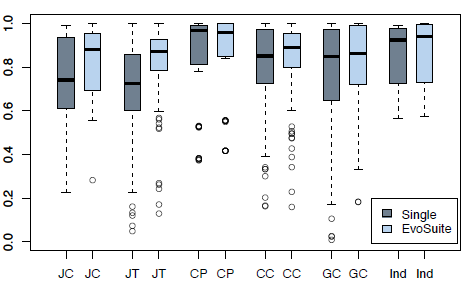
\includegraphics[scale=0.7]{imagens/imagem1.png}
  \label{figura_cobertura}
  \caption{Média de cobertura: Mesmo com limite de evolução de 1 000 000 instruções,\textit{EvoSuite} alcançou cobertura superior \cite{fraser2011evolutionary}}
 %\legend{Fonte: %\cite{fraser2011evosuite} }
\end{figure}

Já em \cite{fraser20151600}, foram testados 100 projetos de código aberto selecionados aleatoriamente no \textit{EvoSuite}, a fim de avaliar a escalabilidade quando existem vários testes. Os autores mostram que o \textit{EvoSuite} é capaz de exercitar oráculos automatizados e produzir alta cobertura de testes ao mesmo tempo. Nos experimentos foram encontrados 32594 falhas distintas em 8844 classes, tal que 1694 dessas falhas podem ser consideradas como falhas reais \cite{fraser20151600}.


% \newpage

\section{Meta-Heurísticas} \label{MetaHeuristicas}

Meta-heurística é um subcampo primário da otimização estocástica, que consiste de algoritmos e técnicas que empregam algum grau de aleatoriedade para encontrar a solução ótima (ou a melhor possível) para problemas reconhecidamente difíceis. \cite{luke2009essentials} \cite{luke2009essentials} ressalva que meta-heurística é um termo que pode gerar desentendimentos
uma vez que não se trata de heuristica sobre (ou para) heurísticas, o que não é necessariamente verdade para todos os algoritmos.  

As próximas secções descrevem as meta-heurísticas que iremos utiliza ou tentar utilizar no problema de teste de software com o \textit{Evosuite}.

\subsection{Colonia de formigas}

Uma meta-heurista bio-inspirada que pode ser útil para o nosso projeto é Colônia de Formigas \cite{dorigo1999ant} ( do inglês \textit{Ant Colony Optimization} ) que surgiu da observação do
comportamento das formigas reais e incluso técnicas de busca local posteriormente. Utiliza algoritmo guloso para para construir a solução inicial e para soluções viáveis. Outro ponto
importante é a quantidade de feromônio depositado pelas formigas que dá a visibilidade que é a capacidade dada às formigas de observar os elementos que compõem a solução ou o caminho que
elas estão percorrendo.





\subsection{Colonia de abelhas}

\subsection{Enxame de partículas}

\subsection{Algoritmo Genético}
\label{sec:alg_genetic}



Um algoritmo genético simula a seleção natural, onde cada indivíduo compete com os outros para sobreviver com base em sua aptidão (\emph{fitness}). Os indivíduos que sobrevivem ao passo de
seleção passam por operações genéticas (cruzamentos e mutações), simulando o que ocorre na biologia, para assim criar uma nova população.

    \subsubsection{Método de seleção de indivíduos}

        Torneio funciona que até que se tenha cromossomos suficientes para fazer a recombinação, nesse caso 4, dois cromossomos são escolhidos aleatoriamente da população, usando uma distribuição de
        probabilidade uniforme, e o de melhor \textit{fitness} é selecionado para o processo de recombinação.

    \subsubsection{Método de \textit{crossover}}

        Operador de \textit{crossover} $C1$ são dados dois pais, $p_1$ e $p_2$, é escolhido um ponto de corte até o qual o filho será igual ao $p_1$. Então, os elementos que faltarem no
        cromossomo filho (todos os clientes faltantes até o ponto de corte) são inseridos no filho seguindo a ordem em que aparecem em $p_2$. 

        Operador de \textit{crossover} do tipo \emph{crossover OX}, por se tratar de um cruzamento para codificação de permutação que, além de ser simples, exige um baixo custo computacional
        quando comparado com os outros esquemas de recombinação para a representação de permutação, desta maneira um maior número de recombinações são possíveis para um tempo fixo de processamento
        da simulação. 

        Outro método de \textit{crossover} de dois indivíduos $A$ e $B$ é usando \textit{crossover} de dois pontos, que é feito selecionando-se aleatoriamente $2$ locus nas posições $L$ e $R$,
        com $L < R$, para serem os pontos da troca.  O primeiro indivíduo é gerado a partir da fusão entre as posições $[0, L]$ e $]R, size(A) - 1]$ de $A$ e as posições $]L, R]$ de $B$, já
        o segundo indivíduo é gerado a partir das posições $[0, L]$ e $]R, size(B) - 1]$ de $B$ e as posições $]L, R]$ de $A$.

        Por fim, o \textit{Uniform Crossover} em vez de escolher aleatoriamente dois pontos de cruzamento, a cada locus, um pai é escolhido aleatoriamente para ter seu alelo copiado; o alelo
        deste pai é copiado para o primeiro descendente enquanto o alelo do outro pai do mesmo locus é copiado para o segundo descendente.

        Da mesma maneira que no método de \textit{crossover} de dois pontos, após a criação da nova geração através desta recombinação, todos os descendentes são verificados e, para todo par de locus
        consecutivos com alelos iguais a 1, um destes locus é escolhido aleatoriamente e seu alelo alterado para 0.

        Após o \textit{crossover}, é necessário fazer a correção de possíveis indivíduos inválidos segundo as restrições do problema.

    \subsubsection{Método de mutação}

         Para uma população, são visitados todos os cromossomos e cada um será mutado se for escolhido um número aleatório maior que a taxa de mutação utilizada. Existe um valor $1/m$
         \cite{gendreau2010handbook} que diz ser um valor ideal para mutações, onde $m$ é o tamanho da instância de entrada.
         
        Após a mutação, também é necessário fazer correções, pois pode haver indivíduos inválidos devido às restrições do problema.


    \subsubsection{\emph{Steady-state}}

        Tipicamente, a execução de um algoritmo genético é dividido em gerações que são substituídas (quase que por completo) a cada iteração do algoritmo. No caso do algoritmo genético
        \emph{steady state} apenas alguns indivíduos são substituídos ao final de cada iteração.

        Neste processo, dois pais devem ser selecionados da população atual e um filho deve ser gerado pelo processo de \emph{crossover}. Em seguida, o pior indivíduo dentre ambos os pais e filho é
        removido e os outros dois são realocados (se necessário) na população. Com isso, o conceito de gerações passa a não fazer sentido pois, neste caso, tem-se apenas um filho gerado enquanto o
        resto da população permanece constante.  

    \subsubsection{Manutenção de diversidade}

        Para manter os indivíduos diversos e evitar a convergência muito cedo, pode ser usado uma função que diversifica a população após a seleção de pais, criação e mutação da geração atual.

        Neste caso, realizam-se testes 2 a 2 em cada indivíduo e se os indivíduos possuírem um número maior que o valor pré-definido (0.5$\%$, por exemplo ) de alelos iguais, o primeiro dos
        dois sofre uma mutação aleatória em um locus.


\subsection{BRKGA}
\label{sec:alg_genetic}

    O BRKGA (biased random-key genetic algorithm)\cite{gonccalves2011biased} é uma metaheuristica para encontrar uma solução ótima ou próxima da ótima. É uma variação do RKGA
    (random-key genetic algorithms) \cite{bean1994genetic} e se obtém uma solução viável para o problema através da decodificação de uma solução codificada. A solução codificada são vetores de
    chaves aleatórias em um intervalo de números reais continuo $(0,1]$ e a decodificação é uma etapa que mapeia um vetor de chaves aleatórias numa solução do problema de otimização e calcula o
    seu custo. Note que o BRKGA tem como seu algoritmo sendo independente do problema. 
    
       \begin{figure}[!htb]
  \centering
 
  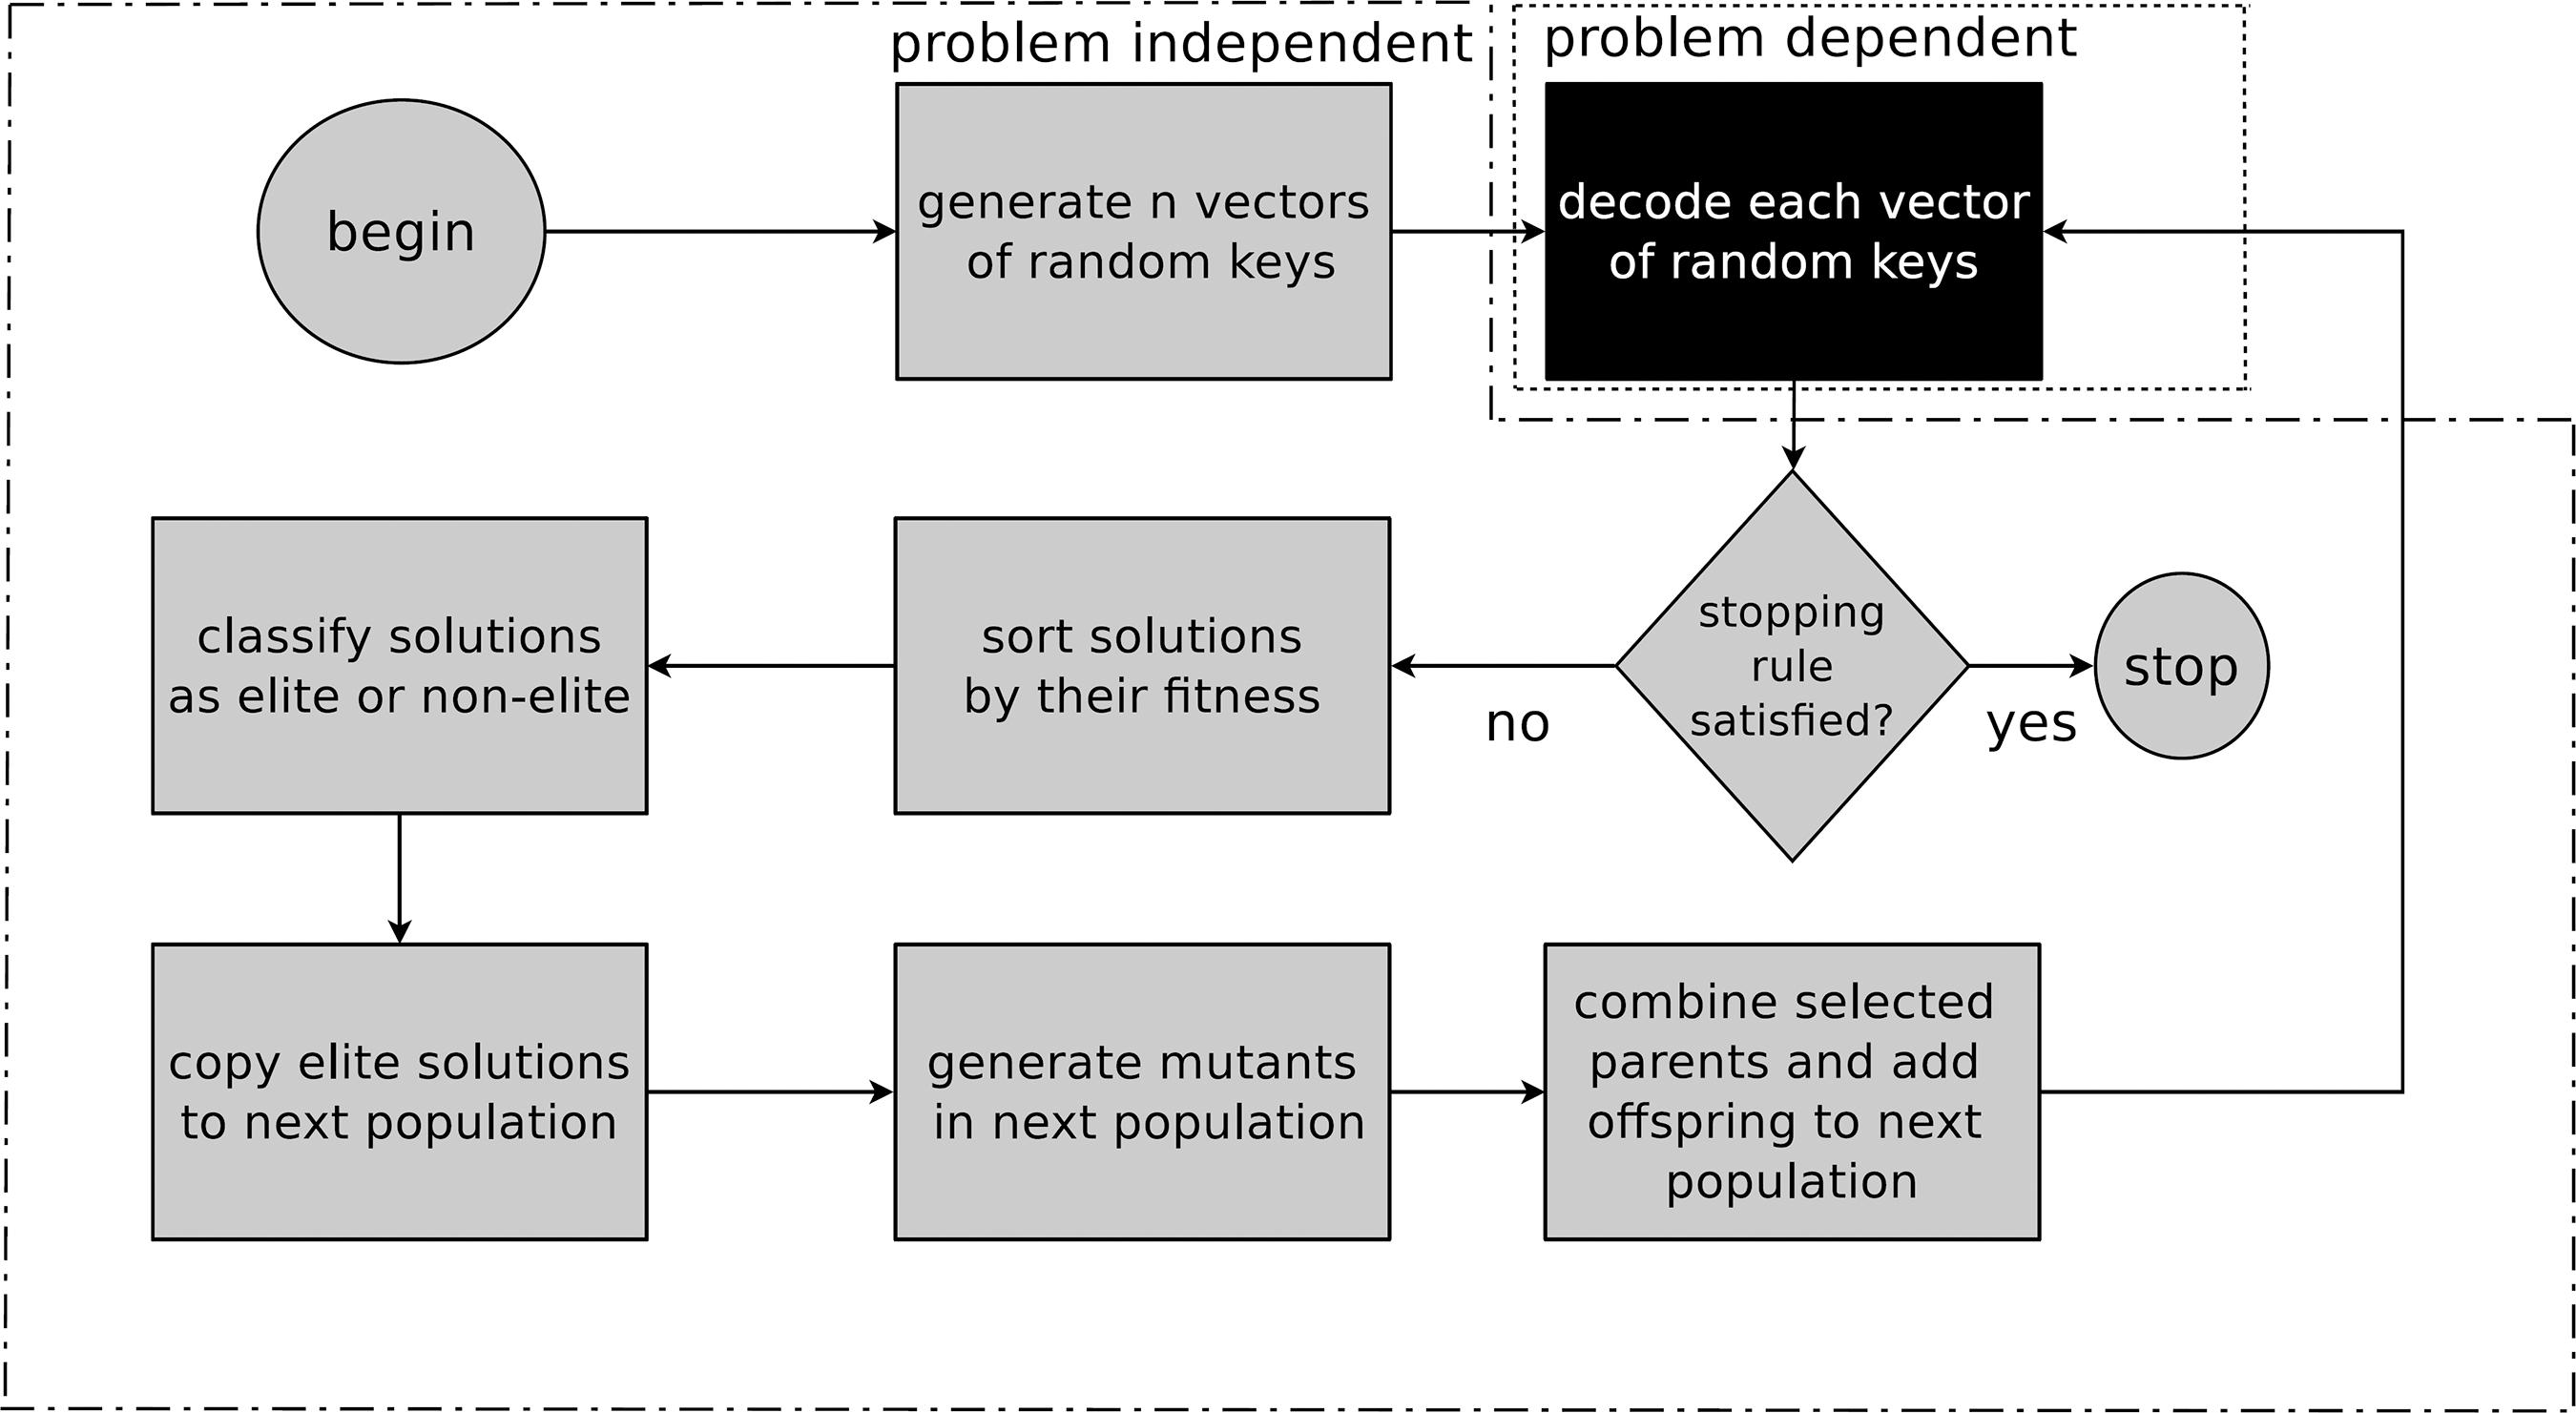
\includegraphics[scale=0.08]{imagens/brkga.jpg}
  \label{figura_brkga}
 \caption{Imagem mostrando o fluxo da meta-heurística BRKGA. \cite{gonccalves2014experimental}}
 %\legend{Fonte: %\cite{fraser2011evosuite} }
\end{figure}

    De forma resumida, a definição de algumas características do BRKGA: 


        \begin{itemize}

        \item Codificação de uma solução com chaves aleatórias em intervalo continuo $[0,1]$ 

        \item Geração de população inicial com $p$ vetores de $n$ chaves aleatórias

        \item Método de seleção de indivíduos é ordenado pelo $fitness$ e gerado dois grupos, elite e não-elite. Após, é escolhido um pai do conjunto elite e o outro é escolhido do conjunto
            não-elite. Com estes é gerado a próxima geração. 

        \end{itemize}

        Todas as variações descritas no algoritmo genético \ref{sec:alg_genetic} são possíveis de se aplicadas no BRKGA. 

\subsection{GRASP}
\label{sec:grasp}

    O GRASP (Greedy Randomized Adaptive Search Procedure) para problemas de otimização combinatória foi introduzida por Feo e Resende \cite{feo1989probabilistic}. O GRASP tem sua iteração
    primeiramente a construção de uma solução inicial a partir de uma heurística construtiva gulosa e aleatória. Depois, é realizado uma busca local com intenção de explorar a vizinhança da
    solução inicial até atingir um mínimo local do espaço de soluções. Após um critério de parada como quantidade de iterações ou tempo de processamento o GRASP devolve a melhor solução
    encontrada e termina sua execução.


    \begin{figure}[!htb]
  \centering
 
  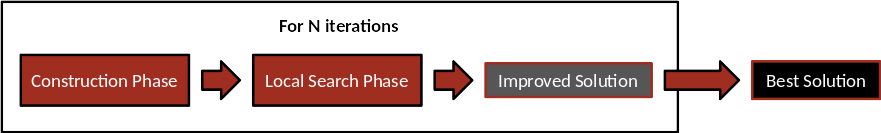
\includegraphics[scale=0.35]{imagens/grasp.png}
  \label{figura_grasp}
 \caption{Imagem ilustrativa de todo o processo da meta-heurística GRASP. \cite{fraser2013whole}}
 %\legend{Fonte: %\cite{fraser2011evosuite} }
\end{figure}

    Algumas variações que podem ser aplicadas:
    \begin{enumerate}

        \item \textbf{Reactive GRASP}: A próxima escolha entre aleatório ou guloso fica definida pelas iterações anteriores e não originalmente que é sempre aleatória;

        \item \textbf{POP in Construction}: Aplicando busca local durante a fase de construção com o principio de que boas soluções estão mais provavelmente próximas a melhores soluções.

        \item \textbf{Busca Tabu}: Podemos usar a Busca Tabu como processo de busca local do GRASP.
    \end{enumerate}




\subsection{Busca Tabu}
\label{sec:busca_tabu}

    A Busca Tabu é uma busca local que permite movimentos que podem não melhorar a solução atual. Para evitar ciclos, existe um mecanismo chamado lista tabu onde os últimos movimentos realizados
    ficam armazenados por um dado número de iterações, chamado \textit{tenure}. Os movimentos que estão na lista de tabus ficam proibidos, a menos que um dado critério de aspiração seja
    satisfeito. Caso um critério de aspiração seja satisfeito o movimento é permitido. A heurística foi originalmente proposta por \cite{glover1986future} \cite{glover1986future} e nos
    últimos 20 anos centenas de artigos utilizam Busca Tabu em diversos problemas de combinatória e mostrando ser bastante eficaz com resultados bem próximos do ótimo ou conseguindo o ótimo
    \cite{gendreau2010handbook}.

    Na Busca Tabu precisamos definir muito bem o espaço de busca e a estrutura da vizinhança. Definir os critérios da restrição de movimentos. Pode ser complicado deixar a meta-heurística
    suficientemente genética para ser usada no \emph{EvoSuite}, porém podemos pensar em casos não muito gerais e aplicar mecanismos de busca por intensificação e por diversidade.

    \begin{figure}[!htb]
  \centering
 
  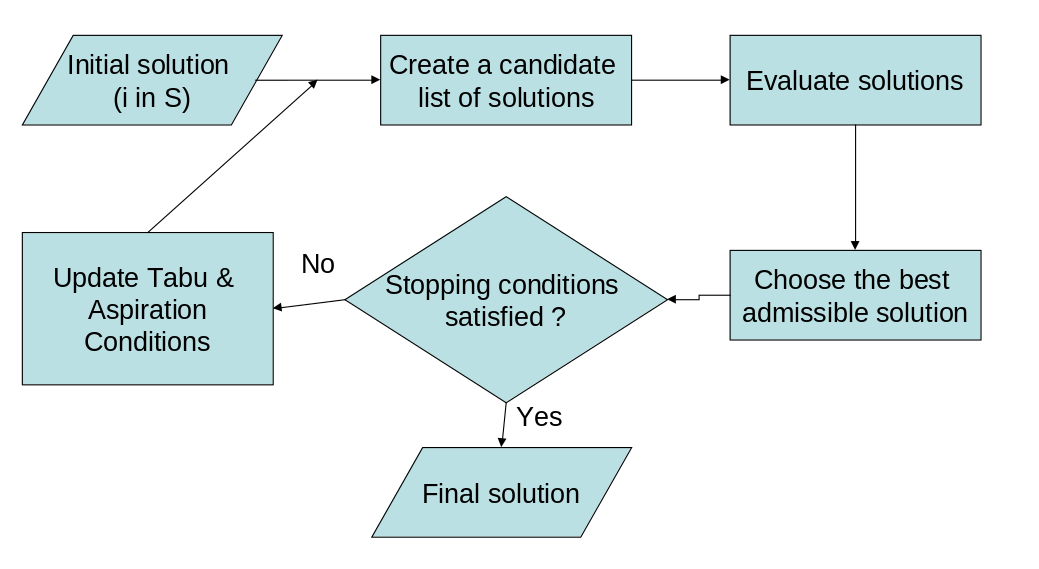
\includegraphics[scale=0.25]{imagens/busca-tabu.png}
  \label{figura_tabu}
 \caption{Imagem ilustrativa de todo o processo da meta-heurística Busca Tabu. \cite{fraser2013whole}}
 %\legend{Fonte: %\cite{fraser2011evosuite} }
\end{figure}

    \subsubsection{Intensificação}

        Uma possível intensificação por vizinhança é que no qual são explorados todos os movimentos possíveis (inserção, remoção e troca) com quaisquer três elementos. 

    \subsubsection{Método de Busca Local}

        \begin{itemize}

        \item {\it Best Improving:} onde toda a exploração da vizinhança de uma solução é dada até a exaustão, ou seja, todos os elementos são analisados até que o mínimo local seja encontrado. Como
            a busca está restrita a vizinhança da solução o mínimo encontrado é local, e não se tem garantida quanto a otimalidade global. No mesmo intuito de buscar por soluções sempre factíveis, a
                fim de não aplicar operadores de reparo nas soluções, a técnica de {\it best improving} só analisa a vizinhança factível. 

        \item {\it First Improving:} a busca na vizinhança é feita usando as técnicas de inserção, remoção e troca. Todas as opções factíveis para as três técnicas são colocadas em uma lista
        e um dos elementos dessa lista é selecionado de forma aleatória, assim que a primeira melhora é encontrada o processo de busca nessa vizinhança para e a lista é atualizada para
        contemplar as novas opções factíveis. 
        \end{itemize}

    \subsubsection{\it Surrogate Objective} 

        Ao resolver um problema por meta-heurísticas, ou ainda, heurísticas, é imprescindível a escolha de uma boa função de avaliação da solução. Por vezes, a melhor escolha para a função de
        avaliação não é a função objetivo, seja porque o calculo da função objetivo tem alto custo computacional ou ainda porque ela não trás informações precisas sobre a solução que está sendo
        tratada. Nesses casos é interessante o uso de uma função de avaliação diferente, conhecida também como {\it surrogate objective}.



    \subsubsection{Diversificação por Reinício}

        Envolve forçar alguns componentes que são raramente utilizados na solução e reiniciar o processo de busca a partir deste ponto.  Seja $t$ o \textit{tenure}, quando a busca é
        reiniciada são colocados os $t$ movimentos mais frequentes no tabu, colocando primeiro o menos frequente e por o último o mais frequente. A frequência é calculada somando 1 cada vez
        que o movimento é realizado pelo operador de busca local. A frequência não é reiniciada quando a busca recomeça. Quando a busca reinicia uma nova solução inicial é construída.

\bibliography{general}{}
\bibliographystyle{plain}

\end{document}
